
\section{Test Model for testcase01}

this positive test case intends to verify the correctness of the execution of a simple instance of the \msrcode{suDeployAndRun} use case.


\subsection{Test Steps Specification}

	\subsubsection{testcase01-ts01oeCreateSystemAndEnvironment-actMsrCreator.outactMsrCreator.oeCreateSystemAndEnvironment}
	\label{TM-testcase01-ts01oeCreateSystemAndEnvironment-actMsrCreator.outactMsrCreator.oeCreateSystemAndEnvironment}

	The \msrcode{testcase01-ts01oeCreateSystemAndEnvironment-actMsrCreator.outactMsrCreator.oeCreateSystemAndEnvironment} has the following properties:

	\begin{teststepmodel}
		\addheading{Test Step}
		\adddoublerow{ts01oeCreateSystemAndEnvironment}{This test step initializes the system state and environment.}
		
		
		\addrowheading{Test Sent Message}
		\addnumberedsinglerow{TSM}{
		\vspace{-0.5cm}
		\begin{description}
			\item[] \textbf{out:Creator}
			\item[] \textbf{sends to system}
			\item[] \textbf{\hyperlink{actMsrCreator.outactMsrCreator.oeCreateSystemAndEnvironment}{actMsrCreator.outactMsrCreator.oeCreateSystemAndEnvironment} (AqtyComCompanies)}
		\end{description}}
		
		
		
		\addrowheading{Variables}
		\addnumbereddoublerow{V}{Creator:icrash.environment.actMsrCreator}
		{only actMsrtCreator actors can trigger the system and environment creation and initialization.}

		\addrowheading{Constraints}
		\addnumberedsinglerow{C}{the number of communication company actor instances present in the environment is equal to four to represent all the communication companies available in Luxembourg.}


		\addrowheading{Oracle Constraints}
		\addnumberedsinglerow{OC}{true for testing only the executability (is available and can be triggered) of the operation.}
	\end{teststepmodel}
	
	
	
		
	% ------------------------------------------
	% MCL Listing
	% ------------------------------------------
	\vspace{1cm}
	The listing~\ref{TM-testcase01-ts01oeCreateSystemAndEnvironment-MCL-LST} provides the \msrmessir (MCL-oriented) specification of the test step.
	
	\scriptsize
	\vspace{0.5cm}
	\begin{lstlisting}[style=MessirStyle,firstnumber=auto,captionpos=b,caption={\msrmessir (MCL-oriented) specification of the test step \emph{testcase01-ts01oeCreateSystemAndEnvironment}.},label=TM-testcase01-ts01oeCreateSystemAndEnvironment-MCL-LST]

	variables{
		Creator:actMsrCreator
		AqtyComCompanies: ptInteger
	}
	
	constraints{
		AqtyComCompanies = 4
	}
	
	oracle{
		constraints{
			true
		}
	}
	
	\end{lstlisting}
	\normalsize 
	
	

	\subsubsection{testcase01-ts02oeSetClock-actActivator.outactActivator.oeSetClock}
	\label{TM-testcase01-ts02oeSetClock-actActivator.outactActivator.oeSetClock}

	The \msrcode{testcase01-ts02oeSetClock-actActivator.outactActivator.oeSetClock} has the following properties:

	\begin{teststepmodel}
		\addheading{Test Step}
		\adddoublerow{ts02oeSetClock}{test the update of the current time.}
		
		
		\addrowheading{Test Sent Message}
		\addnumberedsinglerow{TSM}{
		\vspace{-0.5cm}
		\begin{description}
			\item[] \textbf{out:TheActor}
			\item[] \textbf{sends to system}
			\item[] \textbf{\hyperlink{actActivator.outactActivator.oeSetClock}{actActivator.outactActivator.oeSetClock} (ACurrentClock)}
		\end{description}}
		
		
		
		\addrowheading{Variables}
		\addnumbereddoublerow{V}{TheActor:actActivator}
		{proactive actor responsible of requesting the update of the system's clock.}

		\addrowheading{Constraints}
		\addnumberedsinglerow{C}{TheActor is any instance existing in the current environment status.}
		\addnumberedsinglerow{C}{ACurrentClock is a fixed date equal to the 24th November 2017 at 15:20:00 using a 24-hours notation~\footnote{for more details see the ISO 8601 Data elements and interchange formats � Information interchange � Representation of dates and times - http://www.iso.org/iso/home/standards/iso8601.htm}.}


		\addrowheading{Oracle Constraints}
		\addnumberedsinglerow{OC}{true for testing only the executability (is available and can be triggered) of the operation.}
	\end{teststepmodel}
	
	
	
		
	% ------------------------------------------
	% MCL Listing
	% ------------------------------------------
	\vspace{1cm}
	The listing~\ref{TM-testcase01-ts02oeSetClock-MCL-LST} provides the \msrmessir (MCL-oriented) specification of the test step.
	
	\scriptsize
	\vspace{0.5cm}
	\begin{lstlisting}[style=MessirStyle,firstnumber=auto,captionpos=b,caption={\msrmessir (MCL-oriented) specification of the test step \emph{testcase01-ts02oeSetClock}.},label=TM-testcase01-ts02oeSetClock-MCL-LST]

	variables{
		TheActor:actActivator
		ACurrentClock:dtDateAndTime
	}
	
	constraints{
		TheActor=TheSystem.rnactActivator->any2(true)
		ACurrentClock.date.year.value = 2017
		ACurrentClock.date.month.value = 11
		ACurrentClock.date.day.value = 24
		ACurrentClock.time.hour.value = 15
		ACurrentClock.time.minute.value = 20
		ACurrentClock.time.second.value = 00
	}
	
	oracle{
		constraints{
			true
		}
	}
	
	\end{lstlisting}
	\normalsize 
	
	

	\subsubsection{testcase01-ts03oeLogin-actAdministrator.outactAdministrator.oeLogin}
	\label{TM-testcase01-ts03oeLogin-actAdministrator.outactAdministrator.oeLogin}

	The \msrcode{testcase01-ts03oeLogin-actAdministrator.outactAdministrator.oeLogin} has the following properties:

	\begin{teststepmodel}
		\addheading{Test Step}
		\adddoublerow{ts03oeLogin}{test the authentified access of the administrator}
		
		
		\addrowheading{Test Sent Message}
		\addnumberedsinglerow{TSM}{
		\vspace{-0.5cm}
		\begin{description}
			\item[] \textbf{out:TheActor}
			\item[] \textbf{sends to system}
			\item[] \textbf{\hyperlink{actAdministrator.outactAdministrator.oeLogin}{actAdministrator.outactAdministrator.oeLogin} (AdtLogin, AdtPassword)}
		\end{description}}
		
		
		
		\addrowheading{Variables}
		\addnumbereddoublerow{V}{TheActor:actAdministrator}
		{an actAdministor actor as subtype of actAuthenticated can send oeLogin messages to the system.}

		\addrowheading{Constraints}
		\addnumberedsinglerow{C}{TheActor is any \msrcode{actAdministrator} instance existing in the environment. It is thus expected that there exist at least one.}
		\addnumberedsinglerow{C}{AdtLogin has its value attribute equal to the primitive string 'icrashadmin' (which is the correct administrator login known by the system after the step one.)}
		\addnumberedsinglerow{C}{AdtPassword has its value attribute equal to the primitive string '7WXC1359' (which is the correct administrator password known by the system after the step one.)}


		\addrowheading{Oracle Constraints}
		\addnumberedsinglerow{OC}{the \msrcode{AMessage} value is expected to be equal to the primitive string 'You are logged ! Welcome ...'}
		\addnumberedsinglerow{OC}{TheActor receives from system ieMessage(AMessage)}
	\end{teststepmodel}
	
	
	
		
	% ------------------------------------------
	% MCL Listing
	% ------------------------------------------
	\vspace{1cm}
	The listing~\ref{TM-testcase01-ts03oeLogin-MCL-LST} provides the \msrmessir (MCL-oriented) specification of the test step.
	
	\scriptsize
	\vspace{0.5cm}
	\begin{lstlisting}[style=MessirStyle,firstnumber=auto,captionpos=b,caption={\msrmessir (MCL-oriented) specification of the test step \emph{testcase01-ts03oeLogin}.},label=TM-testcase01-ts03oeLogin-MCL-LST]

	variables{
		TheActor : actAdministrator
		AdtLogin:dtLogin
		AdtPassword:dtPassword
	}
	
	constraints{
		TheActor=TheSystem.rnactAdministrator->any2(true)
		AdtLogin.value.eq('icrashadmin')
		AdtPassword.value.eq('7WXC1359')
	}
	
	oracle{
		variables{
			AMessage:ptString
		}
		constraints{
			AMessage = 'You are logged ! Welcome ...'
			TheActor.inactAdministrator.ieMessage(AMessage)
		}
	}
	
	\end{lstlisting}
	\normalsize 
	
	

	\subsubsection{testcase01-ts04oeAddCoordinator-actAdministrator.outactAdministrator.oeAddCoordinator}
	\label{TM-testcase01-ts04oeAddCoordinator-actAdministrator.outactAdministrator.oeAddCoordinator}

	The \msrcode{testcase01-ts04oeAddCoordinator-actAdministrator.outactAdministrator.oeAddCoordinator} has the following properties:

	\begin{teststepmodel}
		\addheading{Test Step}
		\adddoublerow{ts04oeAddCoordinator}{to test the add of a new coordinator by an administrator.}
		
		
		\addrowheading{Test Sent Message}
		\addnumberedsinglerow{TSM}{
		\vspace{-0.5cm}
		\begin{description}
			\item[] \textbf{out:TheActor}
			\item[] \textbf{sends to system}
			\item[] \textbf{\hyperlink{actAdministrator.outactAdministrator.oeAddCoordinator}{actAdministrator.outactAdministrator.oeAddCoordinator} (AdtCoordinatorID, AdtLogin, AdtPassword)}
		\end{description}}
		
		
		
		\addrowheading{Variables}
		\addnumbereddoublerow{V}{TheActor:actAdministrator}
		{actAdministor actors as being the only one allowed to add coordinators.}

		\addrowheading{Constraints}
		\addnumberedsinglerow{C}{TheActor is any \msrcode{actAdministrator} instance existing in the environment. It is expected that there exists at least one which is the same during all the test case.}
		\addnumberedsinglerow{C}{AdtCoordinatorID is equal to 1 to set the new coordinator ID}
		\addnumberedsinglerow{C}{AdtLogin has its value attribute equal to the primitive string 'steve' which is the ID defined for the new coordinator.}
		\addnumberedsinglerow{C}{AdtPassword has its value attribute equal to the primitive string 'pwdMessirExcalibur2017' which is the password to be set for steve.}


		\addrowheading{Oracle Constraints}
		\addnumberedsinglerow{OC}{the administrator should have been acknowledged for the adding of the new coordinator.}
	\end{teststepmodel}
	
	
	
		
	% ------------------------------------------
	% MCL Listing
	% ------------------------------------------
	\vspace{1cm}
	The listing~\ref{TM-testcase01-ts04oeAddCoordinator-MCL-LST} provides the \msrmessir (MCL-oriented) specification of the test step.
	
	\scriptsize
	\vspace{0.5cm}
	\begin{lstlisting}[style=MessirStyle,firstnumber=auto,captionpos=b,caption={\msrmessir (MCL-oriented) specification of the test step \emph{testcase01-ts04oeAddCoordinator}.},label=TM-testcase01-ts04oeAddCoordinator-MCL-LST]

	variables{
		TheActor : actAdministrator
		AdtCoordinatorID : dtCoordinatorID
		AdtLogin:dtLogin
		AdtPassword:dtPassword
	}
	
	constraints{
		TheActor = TheSystem.rnactAdministrator->any2(true)
		AdtCoordinatorID.value.eq('1')
		AdtLogin.value.eq('steve')
		AdtPassword.value.eq('pwdMessirExcalibur2017')
	}
	
	oracle{
		constraints{
			TheActor.inactAdministrator.ieCoordinatorAdded()
		}
	}
	
	\end{lstlisting}
	\normalsize 
	
	

	\subsubsection{testcase01-ts05oeLogout-actAdministrator.outactAdministrator.oeLogout}
	\label{TM-testcase01-ts05oeLogout-actAdministrator.outactAdministrator.oeLogout}

	The \msrcode{testcase01-ts05oeLogout-actAdministrator.outactAdministrator.oeLogout} has the following properties:

	\begin{teststepmodel}
		\addheading{Test Step}
		\adddoublerow{ts05oeLogout}{to test the loggout of a connected administrator.}
		
		
		\addrowheading{Test Sent Message}
		\addnumberedsinglerow{TSM}{
		\vspace{-0.5cm}
		\begin{description}
			\item[] \textbf{out:TheActor}
			\item[] \textbf{sends to system}
			\item[] \textbf{\hyperlink{actAdministrator.outactAdministrator.oeLogout}{actAdministrator.outactAdministrator.oeLogout} ()}
		\end{description}}
		
		
		
		\addrowheading{Variables}
		\addnumbereddoublerow{V}{TheActor:actAdministrator}
		{an actAdministor actor as subtype of actAuthenticated can send oeLogout messages to the system.}

		\addrowheading{Constraints}
		\addnumberedsinglerow{C}{TheActor is any \msrcode{actAdministrator} instance existing in the environment. It is expected that there exists at least one which is the same during all the test case.}


		\addrowheading{Oracle Constraints}
		\addnumberedsinglerow{OC}{the \msrcode{AMessage} value is expected to be equal to the primitive string 'You are logged out ! Good Bye ...'}
		\addnumberedsinglerow{OC}{the administrator should have received the messahe AMessage.}
	\end{teststepmodel}
	
	
	
		
	% ------------------------------------------
	% MCL Listing
	% ------------------------------------------
	\vspace{1cm}
	The listing~\ref{TM-testcase01-ts05oeLogout-MCL-LST} provides the \msrmessir (MCL-oriented) specification of the test step.
	
	\scriptsize
	\vspace{0.5cm}
	\begin{lstlisting}[style=MessirStyle,firstnumber=auto,captionpos=b,caption={\msrmessir (MCL-oriented) specification of the test step \emph{testcase01-ts05oeLogout}.},label=TM-testcase01-ts05oeLogout-MCL-LST]

	variables{
		TheActor : actAdministrator
	}
	
	constraints{
		TheActor = TheSystem.rnactAdministrator->any2(true)
	}
	
	oracle{
		variables{
			AMessage:ptString
		}
		constraints{
			AMessage = 'You are logged out ! Good Bye ...'
			TheActor.inactAdministrator.ieMessage(AMessage)
		}
	}
	
	\end{lstlisting}
	\normalsize 
	
	

	\subsubsection{testcase01-ts06oeSetClock02-actActivator.outactActivator.oeSetClock}
	\label{TM-testcase01-ts06oeSetClock02-actActivator.outactActivator.oeSetClock}

	The \msrcode{testcase01-ts06oeSetClock02-actActivator.outactActivator.oeSetClock} has the following properties:

	\begin{teststepmodel}
		\addheading{Test Step}
		\adddoublerow{ts06oeSetClock02}{test the update of the current time.}
		
		
		\addrowheading{Test Sent Message}
		\addnumberedsinglerow{TSM}{
		\vspace{-0.5cm}
		\begin{description}
			\item[] \textbf{out:TheActor}
			\item[] \textbf{sends to system}
			\item[] \textbf{\hyperlink{actActivator.outactActivator.oeSetClock}{actActivator.outactActivator.oeSetClock} (ACurrentClock)}
		\end{description}}
		
		
		
		\addrowheading{Variables}
		\addnumbereddoublerow{V}{TheActor:icrash.environment.actActivator}
		{proactive actors responsible of requesting the update of the system's clock.}

		\addrowheading{Constraints}
		\addnumberedsinglerow{C}{TheActor is any instance existing in the current environment status.}
		\addnumberedsinglerow{C}{ACurrentClock is a fixed date equal to the 26th November 2017 at 10:15:00 using a 24-hours notation.}


		\addrowheading{Oracle Constraints}
		\addnumberedsinglerow{OC}{true for testing only the executability (is available and can be triggered) of the operation.}
	\end{teststepmodel}
	
	
	
		
	% ------------------------------------------
	% MCL Listing
	% ------------------------------------------
	\vspace{1cm}
	The listing~\ref{TM-testcase01-ts06oeSetClock02-MCL-LST} provides the \msrmessir (MCL-oriented) specification of the test step.
	
	\scriptsize
	\vspace{0.5cm}
	\begin{lstlisting}[style=MessirStyle,firstnumber=auto,captionpos=b,caption={\msrmessir (MCL-oriented) specification of the test step \emph{testcase01-ts06oeSetClock02}.},label=TM-testcase01-ts06oeSetClock02-MCL-LST]

	variables{
		TheActor:actActivator
		ACurrentClock:dtDateAndTime
	}
	
	constraints{
		TheActor=TheSystem.rnactActivator->any2(true)
		ACurrentClock.date.year.value = 2017
		ACurrentClock.date.month.value = 11
		ACurrentClock.date.day.value = 26
		ACurrentClock.time.hour.value = 10
		ACurrentClock.time.minute.value = 15
		ACurrentClock.time.second.value = 00
	}
	
	oracle{
		constraints{
			true
		}
	}
	
	\end{lstlisting}
	\normalsize 
	
	

	\subsubsection{testcase01-ts07oeAlert1-actComCompany.outactComCompany.oeAlert}
	\label{TM-testcase01-ts07oeAlert1-actComCompany.outactComCompany.oeAlert}

	The \msrcode{testcase01-ts07oeAlert1-actComCompany.outactComCompany.oeAlert} has the following properties:

	\begin{teststepmodel}
		\addheading{Test Step}
		\adddoublerow{ts07oeAlert1}{tests the declaration of a new alert functionality.}
		
		
		\addrowheading{Test Sent Message}
		\addnumberedsinglerow{TSM}{
		\vspace{-0.5cm}
		\begin{description}
			\item[] \textbf{out:TheActor}
			\item[] \textbf{sends to system}
			\item[] \textbf{\hyperlink{actComCompany.outactComCompany.oeAlert}{actComCompany.outactComCompany.oeAlert} (AetHumanKind, AdtDate, AdtTime, AdtPhoneNumber, AdtGPSLocation, AdtComment)}
		\end{description}}
		
		
		
		\addrowheading{Variables}
		\addnumbereddoublerow{V}{TheActor:actComCompany}
		{actComCompany actors transfer alert declaration messages.}

		\addrowheading{Constraints}
		\addnumberedsinglerow{C}{TheActor is any instance existing in the current environment status. It is expected to exist at least one.}
		\addnumberedsinglerow{C}{AetHumanKind is equal to witness}
		\addnumberedsinglerow{C}{AdtDate is equal to the 26th of November 2017}
		\addnumberedsinglerow{C}{AdtTime is equal to 10:10:16 using a 24-hours.}
		\addnumberedsinglerow{C}{AdtPhoneNumber is equal to the ptString value '+3524666445252'.}
		\addnumberedsinglerow{C}{AdtGPSLocation is equal to (49.627675 , 6.159590).}
		\addnumberedsinglerow{C}{AdtComment is equal to '3 cars involved in an accident.'}


		\addrowheading{Oracle Constraints}
		\addnumberedsinglerow{OC}{AdtSMS is equal to the ptString 'Your alert has been registered. We will handle it and keep you informed'.}
		\addnumberedsinglerow{OC}{AdtSMS is sent to the phone number AdtPhoneNumber using the communication company having sent the alert using its ieSmsSend input message.}
	\end{teststepmodel}
	
	
	
		
	% ------------------------------------------
	% MCL Listing
	% ------------------------------------------
	\vspace{1cm}
	The listing~\ref{TM-testcase01-ts07oeAlert1-MCL-LST} provides the \msrmessir (MCL-oriented) specification of the test step.
	
	\scriptsize
	\vspace{0.5cm}
	\begin{lstlisting}[style=MessirStyle,firstnumber=auto,captionpos=b,caption={\msrmessir (MCL-oriented) specification of the test step \emph{testcase01-ts07oeAlert1}.},label=TM-testcase01-ts07oeAlert1-MCL-LST]

	variables{
		TheActor : actComCompany
		AetHumanKind:etHumanKind
		AdtDate:dtDate
		AdtTime:dtTime
		AdtPhoneNumber:dtPhoneNumber
		AdtGPSLocation:dtGPSLocation
		AdtComment:dtComment
	}
	
	constraints{
		TheActor = TheSystem.rnactComCompany->any2(true)
		AetHumanKind = witness
		AdtDate.year.value = 2017
		AdtDate.month.value = 11
		AdtDate.day.value = 26
		AdtTime.hour.value = 10
		AdtTime.minute.value = 10
		AdtTime.second.value = 16
		AdtPhoneNumber.value = '+3524666445252'
		AdtGPSLocation.latitude.value = 49.627675
		AdtGPSLocation.longitude.value = 6.159590
		AdtComment.value = '3 cars involved in an accident.'
	}
	
	oracle{
		variables{
			AdtSMS:dtSMS
		}
		constraints{
			AdtSMS.value = 'Your alert has been registered. We will handle it and keep you informed'
			TheActor.inactComCompany.ieSmsSend(AdtPhoneNumber,AdtSMS)
		}
	}
	
	\end{lstlisting}
	\normalsize 
	
	

	\subsubsection{testcase01-ts08oeSetClock03-actActivator.outactActivator.oeSetClock}
	\label{TM-testcase01-ts08oeSetClock03-actActivator.outactActivator.oeSetClock}

	The \msrcode{testcase01-ts08oeSetClock03-actActivator.outactActivator.oeSetClock} has the following properties:

	\begin{teststepmodel}
		\addheading{Test Step}
		\adddoublerow{ts08oeSetClock03}{test the update of the current time.}
		
		
		\addrowheading{Test Sent Message}
		\addnumberedsinglerow{TSM}{
		\vspace{-0.5cm}
		\begin{description}
			\item[] \textbf{out:TheActor}
			\item[] \textbf{sends to system}
			\item[] \textbf{\hyperlink{actActivator.outactActivator.oeSetClock}{actActivator.outactActivator.oeSetClock} (ACurrentClock)}
		\end{description}}
		
		
		
		\addrowheading{Variables}
		\addnumbereddoublerow{V}{TheActor:actActivator}
		{proactive actor responsible of requesting the update of the system's clock.}

		\addrowheading{Constraints}
		\addnumberedsinglerow{C}{TheActor is any instance existing in the current environment status.}
		\addnumberedsinglerow{C}{ACurrentClock is a fixed date equal to the 26th November 2017 at 10:30:00 using a 24-hours notation.}


		\addrowheading{Oracle Constraints}
		\addnumberedsinglerow{OC}{true for testing only the executability (is available and can be triggered) of the operation.}
	\end{teststepmodel}
	
	
	
		
	% ------------------------------------------
	% MCL Listing
	% ------------------------------------------
	\vspace{1cm}
	The listing~\ref{TM-testcase01-ts08oeSetClock03-MCL-LST} provides the \msrmessir (MCL-oriented) specification of the test step.
	
	\scriptsize
	\vspace{0.5cm}
	\begin{lstlisting}[style=MessirStyle,firstnumber=auto,captionpos=b,caption={\msrmessir (MCL-oriented) specification of the test step \emph{testcase01-ts08oeSetClock03}.},label=TM-testcase01-ts08oeSetClock03-MCL-LST]

	variables{
		TheActor:actActivator
		ACurrentClock:dtDateAndTime
	}
	
	constraints{
		TheActor=TheSystem.rnactActivator->any2(true)
		ACurrentClock.date.year.value = 2017
		ACurrentClock.date.month.value = 11
		ACurrentClock.date.day.value = 26
		ACurrentClock.time.hour.value = 10
		ACurrentClock.time.minute.value = 30
		ACurrentClock.time.second.value = 00
	}
	
	oracle{
		constraints{
			true
		}
	}
	
	\end{lstlisting}
	\normalsize 
	
	

	\subsubsection{testcase01-ts09oeSollicitateCrisisHandling-actActivator.outactActivator.oeSollicitateCrisisHandling}
	\label{TM-testcase01-ts09oeSollicitateCrisisHandling-actActivator.outactActivator.oeSollicitateCrisisHandling}

	The \msrcode{testcase01-ts09oeSollicitateCrisisHandling-actActivator.outactActivator.oeSollicitateCrisisHandling} has the following properties:

	\begin{teststepmodel}
		\addheading{Test Step}
		\adddoublerow{ts09oeSollicitateCrisisHandling}{test the proactive sollication to handle an alert.}
		
		
		\addrowheading{Test Sent Message}
		\addnumberedsinglerow{TSM}{
		\vspace{-0.5cm}
		\begin{description}
			\item[] \textbf{out:TheActor}
			\item[] \textbf{sends to system}
			\item[] \textbf{\hyperlink{actActivator.outactActivator.oeSollicitateCrisisHandling}{actActivator.outactActivator.oeSollicitateCrisisHandling} ()}
		\end{description}}
		
		
		
		\addrowheading{Variables}
		\addnumbereddoublerow{V}{TheActor:icrash.environment.actActivator}
		{proactive actor responsible of triggering sollicitation functionality.}

		\addrowheading{Constraints}
		\addnumberedsinglerow{C}{TheActor is any instance existing in the current environment status. It is expected to exist at least one.}

		\addrowheading{Oracle Variables}
		\addnumbereddoublerow{OV}{TheAdministrator:actAdministrator}
			{actAdministrator actors can be sollicitated to handle alerts.}
		\addnumbereddoublerow{OV}{TheCoordinator:actCoordinator}
			{actCoordinator actors can be sollicitated to handle alerts.}
		\addnumbereddoublerow{OV}{AMessageForCrisisHandlers:ptString}
			{messages sent to sollicitated actors are of type ptString.}

		\addrowheading{Oracle Constraints}
		\addnumberedsinglerow{OC}{TheAdministrator is any instance existing in the current environment status. It is expected to exist at least one.}
		\addnumberedsinglerow{OC}{TheCoordinator is any instance existing in the current environment status. It is expected to exist at least one.}
		\addnumberedsinglerow{OC}{AMessageForCrisisHandlers is equal to the ptString 'There are alerts pending since more than the defined delay. Please REACT !'}
		\addnumberedsinglerow{OC}{TheCoordinator and TheAdministrator have received the message AMessageForCrisisHandlers.}
	\end{teststepmodel}
	
	
	
		
	% ------------------------------------------
	% MCL Listing
	% ------------------------------------------
	\vspace{1cm}
	The listing~\ref{TM-testcase01-ts09oeSollicitateCrisisHandling-MCL-LST} provides the \msrmessir (MCL-oriented) specification of the test step.
	
	\scriptsize
	\vspace{0.5cm}
	\begin{lstlisting}[style=MessirStyle,firstnumber=auto,captionpos=b,caption={\msrmessir (MCL-oriented) specification of the test step \emph{testcase01-ts09oeSollicitateCrisisHandling}.},label=TM-testcase01-ts09oeSollicitateCrisisHandling-MCL-LST]

	variables{
		TheActor : actActivator
	}
	
	constraints{
		TheActor = TheSystem.rnactActivator->any2(true)
	}
	
	oracle{
		variables{
			TheAdministrator:actAdministrator
			TheCoordinator:actCoordinator
			AMessageForCrisisHandlers:ptString
		}
		constraints{
			TheAdministrator = TheSystem.rnactAdministrator->any2(true)
			TheCoordinator = TheSystem.rnactCoordinator->any2(true)
			AMessageForCrisisHandlers = 'There are alerts pending since more than the defined delay. Please REACT !'
			TheAdministrator.inactAdministrator.ieMessage(AMessageForCrisisHandlers)
			TheCoordinator.inactAdministrator.ieMessage(AMessageForCrisisHandlers)
		}
	}
	
	\end{lstlisting}
	\normalsize 
	
	

	\subsubsection{testcase01-ts10oeLogin02-actAuthenticated.outactAuthenticated.oeLogin}
	\label{TM-testcase01-ts10oeLogin02-actAuthenticated.outactAuthenticated.oeLogin}

	The \msrcode{testcase01-ts10oeLogin02-actAuthenticated.outactAuthenticated.oeLogin} has the following properties:

	\begin{teststepmodel}
		\addheading{Test Step}
		\adddoublerow{ts10oeLogin02}{test the authentified access of the coordinator}
		
		
		\addrowheading{Test Sent Message}
		\addnumberedsinglerow{TSM}{
		\vspace{-0.5cm}
		\begin{description}
			\item[] \textbf{out:TheActor}
			\item[] \textbf{sends to system}
			\item[] \textbf{\hyperlink{actAuthenticated.outactAuthenticated.oeLogin}{actAuthenticated.outactAuthenticated.oeLogin} (AdtLogin, AdtPassword)}
		\end{description}}
		
		
		
		\addrowheading{Variables}
		\addnumbereddoublerow{V}{TheActor:actCoordinator}
		{an actCoordinator actor as subtype of actAuthenticated can send oeLogin messages to the system.}

		\addrowheading{Constraints}
		\addnumberedsinglerow{C}{TheActor is any \msrcode{actAdministrator} instance existing in the environment. It is thus expected that there exist at least one.}
		\addnumberedsinglerow{C}{AdtLogin has its value attribute equal to the primitive string 'icrashadmin' (which is the correct administrator login known by the system after the step one.)}
		\addnumberedsinglerow{C}{AdtPassword has its value attribute equal to the primitive string '7WXC1359' (which is the correct administrator password known by the system after the step one.)}


		\addrowheading{Oracle Constraints}
		\addnumberedsinglerow{OC}{the \msrcode{AMessage} value is expected to be equal to the primitive string 'You are logged ! Welcome ...'}
	\end{teststepmodel}
	
	
	
		
	% ------------------------------------------
	% MCL Listing
	% ------------------------------------------
	\vspace{1cm}
	The listing~\ref{TM-testcase01-ts10oeLogin02-MCL-LST} provides the \msrmessir (MCL-oriented) specification of the test step.
	
	\scriptsize
	\vspace{0.5cm}
	\begin{lstlisting}[style=MessirStyle,firstnumber=auto,captionpos=b,caption={\msrmessir (MCL-oriented) specification of the test step \emph{testcase01-ts10oeLogin02}.},label=TM-testcase01-ts10oeLogin02-MCL-LST]

	variables{
		TheActor : actCoordinator
		AdtLogin:dtLogin
		AdtPassword:dtPassword
	}
	
	constraints{
		TheActor = TheSystem.rnactCoordinator->select(a | a.rnctCoordinator.login.value.eq('steve'))->any2(true)
		AdtLogin.value.eq('steve')
		AdtPassword.value.eq('pwdMessirExcalibur2017')
	}
	
	oracle{
		variables{
			AMessage:ptString
		}
		constraints{
			AMessage = 'You are logged ! Welcome ...'
			TheActor.inactAuthenticated.ieMessage(AMessage)
		}
	}
	
	\end{lstlisting}
	\normalsize 
	
	

	\subsubsection{testcase01-ts11oeGetCrisisSet-actCoordinator.outactCoordinator.oeGetCrisisSet}
	\label{TM-testcase01-ts11oeGetCrisisSet-actCoordinator.outactCoordinator.oeGetCrisisSet}

	The \msrcode{testcase01-ts11oeGetCrisisSet-actCoordinator.outactCoordinator.oeGetCrisisSet} has the following properties:

	\begin{teststepmodel}
		\addheading{Test Step}
		\adddoublerow{ts11oeGetCrisisSet}{cf. actor documentation}
		
		
		\addrowheading{Test Sent Message}
		\addnumberedsinglerow{TSM}{
		\vspace{-0.5cm}
		\begin{description}
			\item[] \textbf{out:TheActor}
			\item[] \textbf{sends to system}
			\item[] \textbf{\hyperlink{actCoordinator.outactCoordinator.oeGetCrisisSet}{actCoordinator.outactCoordinator.oeGetCrisisSet} (AetCrisisStatus)}
		\end{description}}
		
		
		
		\addrowheading{Variables}
		\addnumbereddoublerow{V}{TheActor:icrash.environment.actCoordinator}
		{cf. actor documentation}
		\addnumbereddoublerow{V}{AetCrisisStatus:icrash.concepts.primarytypes.datatypes.etCrisisStatus}
		{cf. actor documentation}
		\addnumbereddoublerow{V}{ActCrisis:icrash.concepts.primarytypes.classes.ctCrisis}
		{cf. actor documentation}

		\addrowheading{Constraints}
		\addnumberedsinglerow{C}{TheActor is the coordinator actor related to a coordinator in the system's state having steve as login value}
		\addnumberedsinglerow{C}{AetCrisisStatus value is pending}


		\addrowheading{Oracle Constraints}
		\addnumberedsinglerow{OC}{ActCrisis is any ctCrisis instance that has been sent to TheActor.}
	\end{teststepmodel}
	
	
	
		
	% ------------------------------------------
	% MCL Listing
	% ------------------------------------------
	\vspace{1cm}
	The listing~\ref{TM-testcase01-ts11oeGetCrisisSet-MCL-LST} provides the \msrmessir (MCL-oriented) specification of the test step.
	
	\scriptsize
	\vspace{0.5cm}
	\begin{lstlisting}[style=MessirStyle,firstnumber=auto,captionpos=b,caption={\msrmessir (MCL-oriented) specification of the test step \emph{testcase01-ts11oeGetCrisisSet}.},label=TM-testcase01-ts11oeGetCrisisSet-MCL-LST]

	variables{
		TheActor : actCoordinator
		AetCrisisStatus : etCrisisStatus
	}
	
	constraints{
		TheActor=TheSystem.rnactCoordinator
		            ->select(a | a.rnctCoordinator.login.value.eq('steve'))
		            ->any2(true)
		AetCrisisStatus = pending
	}
	
	oracle{
		variables{
			ActCrisis:ctCrisis
		}
		constraints{
			TheActor.inactCoordinator.ieSendACrisis(ActCrisis)
		}
	}
	
	\end{lstlisting}
	\normalsize 
	
	

	\subsubsection{testcase01-ts12oeSetCrisisHandler-actCoordinator.outactCoordinator.oeSetCrisisHandler}
	\label{TM-testcase01-ts12oeSetCrisisHandler-actCoordinator.outactCoordinator.oeSetCrisisHandler}

	The \msrcode{testcase01-ts12oeSetCrisisHandler-actCoordinator.outactCoordinator.oeSetCrisisHandler} has the following properties:

	\begin{teststepmodel}
		\addheading{Test Step}
		\adddoublerow{ts12oeSetCrisisHandler}{cf. actor documentation}
		
		
		\addrowheading{Test Sent Message}
		\addnumberedsinglerow{TSM}{
		\vspace{-0.5cm}
		\begin{description}
			\item[] \textbf{out:TheActor}
			\item[] \textbf{sends to system}
			\item[] \textbf{\hyperlink{actCoordinator.outactCoordinator.oeSetCrisisHandler}{actCoordinator.outactCoordinator.oeSetCrisisHandler} (AdtCrisisID)}
		\end{description}}
		
		
		
		\addrowheading{Variables}
		\addnumbereddoublerow{V}{TheActor:icrash.environment.actCoordinator}
		{cf. actor documentation}
		\addnumbereddoublerow{V}{TheComCompany:icrash.environment.actComCompany}
		{cf. actor documentation}
		\addnumbereddoublerow{V}{TheCoordinator:icrash.environment.actCoordinator}
		{cf. actor documentation}
		\addnumbereddoublerow{V}{AdtCrisisID:icrash.concepts.primarytypes.datatypes.dtCrisisID}
		{cf. actor documentation}
		\addnumbereddoublerow{V}{AMessage:lu.uni.lassy.messir.libraries.primitives.ptString}
		{cf. actor documentation}
		\addnumbereddoublerow{V}{AdtPhoneNumber:icrash.concepts.primarytypes.datatypes.dtPhoneNumber}
		{cf. actor documentation}
		\addnumbereddoublerow{V}{AdtSMS:icrash.concepts.secondarytypes.datatypes.dtSMS}
		{cf. actor documentation}
		\addnumbereddoublerow{V}{ActAlert:icrash.concepts.primarytypes.classes.ctAlert}
		{cf. actor documentation}

		\addrowheading{Constraints}
		\addnumberedsinglerow{C}{TheActor is the coordinator actor related to a coordinator in the system's state having steve as login value}
		\addnumberedsinglerow{C}{AdtCrisisID as a value of 1}
		\addnumberedsinglerow{C}{AMessage is the string 'You are now considered as handling the crisis !'
		}
		\addnumberedsinglerow{C}{AdtPhoneNumber}
		\addnumberedsinglerow{C}{AdtSMS has for value the string 'The handling of your alert by our services is in progress !'
		}


		\addrowheading{Oracle Constraints}
		\addnumberedsinglerow{OC}{there is a communication company actor that received the message ieSmsSend(AdtPhoneNumber,AdtSMS)}
		\addnumberedsinglerow{OC}{there is a coordinator actor that received an alert using the message ieSendAnAlert(ActAlert)}
	\end{teststepmodel}
	
	
	
		
	% ------------------------------------------
	% MCL Listing
	% ------------------------------------------
	\vspace{1cm}
	The listing~\ref{TM-testcase01-ts12oeSetCrisisHandler-MCL-LST} provides the \msrmessir (MCL-oriented) specification of the test step.
	
	\scriptsize
	\vspace{0.5cm}
	\begin{lstlisting}[style=MessirStyle,firstnumber=auto,captionpos=b,caption={\msrmessir (MCL-oriented) specification of the test step \emph{testcase01-ts12oeSetCrisisHandler}.},label=TM-testcase01-ts12oeSetCrisisHandler-MCL-LST]

	variables{
		TheActor : actCoordinator
		AdtCrisisID : dtCrisisID
	}
	
	constraints{
		TheActor=TheSystem.rnactCoordinator
		            ->select(a | a.rnctCoordinator.login.value.eq('steve'))
		            ->any2(true)
	}
	
	oracle{
		variables{
			AMessage:ptString
			AdtPhoneNumber:dtPhoneNumber
			AdtSMS:dtSMS
			ActAlert:ctAlert
			TheComCompany: actComCompany
			TheCoordinator:actCoordinator
		}
		constraints{
			AMessage = 'You are now considered as handling the crisis !'
			AdtSMS.value = 'The handling of your alert by our services is in progress !'
			TheComCompany.inactComCompany.ieSmsSend(AdtPhoneNumber,AdtSMS)
			TheCoordinator.inactCoordinator.ieSendAnAlert(ActAlert)
			TheActor.inactAuthenticated.ieMessage(AMessage)
		}
	}
	
	\end{lstlisting}
	\normalsize 
	
	

	\subsubsection{testcase01-ts13oeSetClock04-actActivator.outactActivator.oeSetClock}
	\label{TM-testcase01-ts13oeSetClock04-actActivator.outactActivator.oeSetClock}

	The \msrcode{testcase01-ts13oeSetClock04-actActivator.outactActivator.oeSetClock} has the following properties:

	\begin{teststepmodel}
		\addheading{Test Step}
		\adddoublerow{ts13oeSetClock04}{cf. actor documentation}
		
		
		\addrowheading{Test Sent Message}
		\addnumberedsinglerow{TSM}{
		\vspace{-0.5cm}
		\begin{description}
			\item[] \textbf{out:TheActor}
			\item[] \textbf{sends to system}
			\item[] \textbf{\hyperlink{actActivator.outactActivator.oeSetClock}{actActivator.outactActivator.oeSetClock} (ACurrentClock)}
		\end{description}}
		
		
		
		\addrowheading{Variables}
		\addnumbereddoublerow{V}{TheActor:icrash.environment.actActivator}
		{cf. actor documentation}
		\addnumbereddoublerow{V}{ACurrentClock:lu.uni.lassy.messir.libraries.calendar.dtDateAndTime}
		{cf. actor documentation}

		\addrowheading{Constraints}
		\addnumberedsinglerow{C}{TheActor}
		\addnumberedsinglerow{C}{ACurrentClock}


	\end{teststepmodel}
	
	
	
		
	% ------------------------------------------
	% MCL Listing
	% ------------------------------------------
	\vspace{1cm}
	The listing~\ref{TM-testcase01-ts13oeSetClock04-MCL-LST} provides the \msrmessir (MCL-oriented) specification of the test step.
	
	\scriptsize
	\vspace{0.5cm}
	\begin{lstlisting}[style=MessirStyle,firstnumber=auto,captionpos=b,caption={\msrmessir (MCL-oriented) specification of the test step \emph{testcase01-ts13oeSetClock04}.},label=TM-testcase01-ts13oeSetClock04-MCL-LST]

	variables{
		TheActor:actActivator
		ACurrentClock:dtDateAndTime
	}
	
	constraints{
		TheActor=TheSystem.rnactActivator->any2(true)
		ACurrentClock.date.year.value = 2017
		ACurrentClock.date.month.value = 11
		ACurrentClock.date.day.value = 26
		ACurrentClock.time.hour.value = 10
		ACurrentClock.time.minute.value = 45
		ACurrentClock.time.second.value = 00
	}
	
	oracle{
		constraints{
			true
		}
	}
	
	\end{lstlisting}
	\normalsize 
	
	

	\subsubsection{testcase01-ts14oeValidateAlert-actCoordinator.outactCoordinator.oeValidateAlert}
	\label{TM-testcase01-ts14oeValidateAlert-actCoordinator.outactCoordinator.oeValidateAlert}

	The \msrcode{testcase01-ts14oeValidateAlert-actCoordinator.outactCoordinator.oeValidateAlert} has the following properties:

	\begin{teststepmodel}
		\addheading{Test Step}
		\adddoublerow{ts14oeValidateAlert}{cf. actor documentation}
		
		
		\addrowheading{Test Sent Message}
		\addnumberedsinglerow{TSM}{
		\vspace{-0.5cm}
		\begin{description}
			\item[] \textbf{out:TheActor}
			\item[] \textbf{sends to system}
			\item[] \textbf{\hyperlink{actCoordinator.outactCoordinator.oeValidateAlert}{actCoordinator.outactCoordinator.oeValidateAlert} (AdtAlertID)}
		\end{description}}
		
		
		
		\addrowheading{Variables}
		\addnumbereddoublerow{V}{TheActor:icrash.environment.actCoordinator}
		{cf. actor documentation}
		\addnumbereddoublerow{V}{AdtAlertID:icrash.concepts.primarytypes.datatypes.dtAlertID}
		{cf. actor documentation}
		\addnumbereddoublerow{V}{AMessage:lu.uni.lassy.messir.libraries.primitives.ptString}
		{cf. actor documentation}

		\addrowheading{Constraints}
		\addnumberedsinglerow{C}{TheActor is the coordinator actor related to a coordinator in the system's state having steve as login value}
		\addnumberedsinglerow{C}{AdtAlertID}
		\addnumberedsinglerow{C}{AMessage}


		\addrowheading{Oracle Constraints}
		\addnumberedsinglerow{OC}{}
	\end{teststepmodel}
	
	
	
		
	% ------------------------------------------
	% MCL Listing
	% ------------------------------------------
	\vspace{1cm}
	The listing~\ref{TM-testcase01-ts14oeValidateAlert-MCL-LST} provides the \msrmessir (MCL-oriented) specification of the test step.
	
	\scriptsize
	\vspace{0.5cm}
	\begin{lstlisting}[style=MessirStyle,firstnumber=auto,captionpos=b,caption={\msrmessir (MCL-oriented) specification of the test step \emph{testcase01-ts14oeValidateAlert}.},label=TM-testcase01-ts14oeValidateAlert-MCL-LST]

	variables{
		TheActor : actCoordinator
		AdtAlertID : dtAlertID
	}
	
	constraints{
		TheActor=TheSystem.rnactCoordinator
		            ->select(a | a.rnctCoordinator.login.value.eq('steve'))
		            ->any2(true)
	}
	
	oracle{
		variables{
			AMessage:ptString
		}
		constraints{
			AMessage = 'The Alert is now declared as valid !'
			TheActor.actAuthenticated.inactAuthenticated.ieMessage(AMessage)
		}
	}
	
	\end{lstlisting}
	\normalsize 
	
	

	\subsubsection{testcase01-ts15oeAlert2-actComCompany.outactComCompany.oeAlert}
	\label{TM-testcase01-ts15oeAlert2-actComCompany.outactComCompany.oeAlert}

	The \msrcode{testcase01-ts15oeAlert2-actComCompany.outactComCompany.oeAlert} has the following properties:

	\begin{teststepmodel}
		\addheading{Test Step}
		\adddoublerow{ts15oeAlert2}{cf. actor documentation}
		
		
		\addrowheading{Test Sent Message}
		\addnumberedsinglerow{TSM}{
		\vspace{-0.5cm}
		\begin{description}
			\item[] \textbf{out:TheActor}
			\item[] \textbf{sends to system}
			\item[] \textbf{\hyperlink{actComCompany.outactComCompany.oeAlert}{actComCompany.outactComCompany.oeAlert} (AetHumanKind, AdtDate, AdtTime, AdtPhoneNumber, AdtGPSLocation, AdtComment)}
		\end{description}}
		
		
		
		\addrowheading{Variables}
		\addnumbereddoublerow{V}{TheActor:icrash.environment.actComCompany}
		{cf. actor documentation}
		\addnumbereddoublerow{V}{AetHumanKind:icrash.concepts.primarytypes.datatypes.etHumanKind}
		{cf. actor documentation}
		\addnumbereddoublerow{V}{AdtDate:lu.uni.lassy.messir.libraries.calendar.dtDate}
		{cf. actor documentation}
		\addnumbereddoublerow{V}{AdtTime:lu.uni.lassy.messir.libraries.calendar.dtTime}
		{cf. actor documentation}
		\addnumbereddoublerow{V}{AdtPhoneNumber:icrash.concepts.primarytypes.datatypes.dtPhoneNumber}
		{cf. actor documentation}
		\addnumbereddoublerow{V}{AdtGPSLocation:icrash.concepts.primarytypes.datatypes.dtGPSLocation}
		{cf. actor documentation}
		\addnumbereddoublerow{V}{AdtComment:icrash.concepts.primarytypes.datatypes.dtComment}
		{cf. actor documentation}
		\addnumbereddoublerow{V}{AdtSMS:icrash.concepts.secondarytypes.datatypes.dtSMS}
		{cf. actor documentation}

		\addrowheading{Constraints}
		\addnumberedsinglerow{C}{TheActor}
		\addnumberedsinglerow{C}{AetHumanKind}
		\addnumberedsinglerow{C}{AdtDate}
		\addnumberedsinglerow{C}{AdtTime}
		\addnumberedsinglerow{C}{AdtPhoneNumber}
		\addnumberedsinglerow{C}{AdtGPSLocation}
		\addnumberedsinglerow{C}{AdtComment}
		\addnumberedsinglerow{C}{AdtSMS}


		\addrowheading{Oracle Constraints}
		\addnumberedsinglerow{OC}{}
	\end{teststepmodel}
	
	
	
		
	% ------------------------------------------
	% MCL Listing
	% ------------------------------------------
	\vspace{1cm}
	The listing~\ref{TM-testcase01-ts15oeAlert2-MCL-LST} provides the \msrmessir (MCL-oriented) specification of the test step.
	
	\scriptsize
	\vspace{0.5cm}
	\begin{lstlisting}[style=MessirStyle,firstnumber=auto,captionpos=b,caption={\msrmessir (MCL-oriented) specification of the test step \emph{testcase01-ts15oeAlert2}.},label=TM-testcase01-ts15oeAlert2-MCL-LST]

	variables{
		TheActor : actComCompany
		AetHumanKind:etHumanKind
		AdtDate:dtDate
		AdtTime:dtTime
		AdtPhoneNumber:dtPhoneNumber
		AdtGPSLocation:dtGPSLocation
		AdtComment:dtComment
	}
	
	constraints{
		TheActor = TheSystem.rnactComCompany->any2(true)
		AetHumanKind = witness
		AdtDate.year.value = 2017
		AdtDate.month.value = 11
		AdtDate.day.value = 26
		AdtTime.hour.value = 10
		AdtTime.minute.value = 20
		AdtTime.second.value = 00
		AdtPhoneNumber.value = '+3524666445000'
		AdtGPSLocation.latitude.value = 49.627095
		AdtGPSLocation.longitude.value = 6.160251
		AdtComment.value = 'A car crash just happened.'
	}
	
	oracle{
		variables{
			AdtSMS:dtSMS
		}
		constraints{
			AdtSMS.value = 'Your alert has been registered. We will handle it and keep you informed'
			TheActor.actComCompany.inactComCompany.ieSmsSend(AdtPhoneNumber,AdtSMS)
		}
	}
	
	\end{lstlisting}
	\normalsize 
	
	

	\subsubsection{testcase01-ts16oeSetClock05-actActivator.outactActivator.oeSetClock}
	\label{TM-testcase01-ts16oeSetClock05-actActivator.outactActivator.oeSetClock}

	The \msrcode{testcase01-ts16oeSetClock05-actActivator.outactActivator.oeSetClock} has the following properties:

	\begin{teststepmodel}
		\addheading{Test Step}
		\adddoublerow{ts16oeSetClock05}{cf. actor documentation}
		
		
		\addrowheading{Test Sent Message}
		\addnumberedsinglerow{TSM}{
		\vspace{-0.5cm}
		\begin{description}
			\item[] \textbf{out:TheActor}
			\item[] \textbf{sends to system}
			\item[] \textbf{\hyperlink{actActivator.outactActivator.oeSetClock}{actActivator.outactActivator.oeSetClock} (ACurrentClock)}
		\end{description}}
		
		
		
		\addrowheading{Variables}
		\addnumbereddoublerow{V}{TheActor:icrash.environment.actActivator}
		{cf. actor documentation}
		\addnumbereddoublerow{V}{ACurrentClock:lu.uni.lassy.messir.libraries.calendar.dtDateAndTime}
		{cf. actor documentation}

		\addrowheading{Constraints}
		\addnumberedsinglerow{C}{TheActor}
		\addnumberedsinglerow{C}{ACurrentClock}


	\end{teststepmodel}
	
	
	
		
	% ------------------------------------------
	% MCL Listing
	% ------------------------------------------
	\vspace{1cm}
	The listing~\ref{TM-testcase01-ts16oeSetClock05-MCL-LST} provides the \msrmessir (MCL-oriented) specification of the test step.
	
	\scriptsize
	\vspace{0.5cm}
	\begin{lstlisting}[style=MessirStyle,firstnumber=auto,captionpos=b,caption={\msrmessir (MCL-oriented) specification of the test step \emph{testcase01-ts16oeSetClock05}.},label=TM-testcase01-ts16oeSetClock05-MCL-LST]

	variables{
		TheActor:actActivator
		ACurrentClock:dtDateAndTime
	}
	
	constraints{
		TheActor=TheSystem.rnactActivator->any2(true)
		ACurrentClock.date.year.value = 2017
		ACurrentClock.date.month.value = 11
		ACurrentClock.date.day.value = 26
		ACurrentClock.time.hour.value = 12
		ACurrentClock.time.minute.value = 45
		ACurrentClock.time.second.value = 00
	}
	
	oracle{
		constraints{
			true
		}
	}
	
	\end{lstlisting}
	\normalsize 
	
	

	\subsubsection{testcase01-ts17oeSetCrisisStatus-actCoordinator.outactCoordinator.oeSetCrisisStatus}
	\label{TM-testcase01-ts17oeSetCrisisStatus-actCoordinator.outactCoordinator.oeSetCrisisStatus}

	The \msrcode{testcase01-ts17oeSetCrisisStatus-actCoordinator.outactCoordinator.oeSetCrisisStatus} has the following properties:

	\begin{teststepmodel}
		\addheading{Test Step}
		\adddoublerow{ts17oeSetCrisisStatus}{cf. actor documentation}
		
		
		\addrowheading{Test Sent Message}
		\addnumberedsinglerow{TSM}{
		\vspace{-0.5cm}
		\begin{description}
			\item[] \textbf{out:TheActor}
			\item[] \textbf{sends to system}
			\item[] \textbf{\hyperlink{actCoordinator.outactCoordinator.oeSetCrisisStatus}{actCoordinator.outactCoordinator.oeSetCrisisStatus} (AdtCrisisID, AetCrisisStatus)}
		\end{description}}
		
		
		
		\addrowheading{Variables}
		\addnumbereddoublerow{V}{TheActor:icrash.environment.actCoordinator}
		{cf. actor documentation}
		\addnumbereddoublerow{V}{AdtCrisisID:icrash.concepts.primarytypes.datatypes.dtCrisisID}
		{cf. actor documentation}
		\addnumbereddoublerow{V}{AetCrisisStatus:icrash.concepts.primarytypes.datatypes.etCrisisStatus}
		{cf. actor documentation}
		\addnumbereddoublerow{V}{AMessage:lu.uni.lassy.messir.libraries.primitives.ptString}
		{cf. actor documentation}

		\addrowheading{Constraints}
		\addnumberedsinglerow{C}{TheActor is the coordinator actor related to a coordinator in the system's state having steve as login value}
		\addnumberedsinglerow{C}{AdtCrisisID}
		\addnumberedsinglerow{C}{AetCrisisStatus}
		\addnumberedsinglerow{C}{AMessage}


		\addrowheading{Oracle Constraints}
		\addnumberedsinglerow{OC}{}
	\end{teststepmodel}
	
	
	
		
	% ------------------------------------------
	% MCL Listing
	% ------------------------------------------
	\vspace{1cm}
	The listing~\ref{TM-testcase01-ts17oeSetCrisisStatus-MCL-LST} provides the \msrmessir (MCL-oriented) specification of the test step.
	
	\scriptsize
	\vspace{0.5cm}
	\begin{lstlisting}[style=MessirStyle,firstnumber=auto,captionpos=b,caption={\msrmessir (MCL-oriented) specification of the test step \emph{testcase01-ts17oeSetCrisisStatus}.},label=TM-testcase01-ts17oeSetCrisisStatus-MCL-LST]

	variables{
		TheActor : actCoordinator
		AdtCrisisID : dtCrisisID
		AetCrisisStatus : etCrisisStatus
	}
	
	constraints{
		TheActor=TheSystem.rnactCoordinator
		            ->select(a | a.rnctCoordinator.login.value.eq('steve'))
		            ->any2(true)
	}
	
	oracle{
		variables{
			AMessage:ptString
		}
		constraints{
			AMessage = 'The crisis status has been updated !'
			TheActor.inactAuthenticated.ieMessage(AMessage)
		}
	}
	
	\end{lstlisting}
	\normalsize 
	
	

	\subsubsection{testcase01-ts18oeReportOnCrisis-actCoordinator.outactCoordinator.oeReportOnCrisis}
	\label{TM-testcase01-ts18oeReportOnCrisis-actCoordinator.outactCoordinator.oeReportOnCrisis}

	The \msrcode{testcase01-ts18oeReportOnCrisis-actCoordinator.outactCoordinator.oeReportOnCrisis} has the following properties:

	\begin{teststepmodel}
		\addheading{Test Step}
		\adddoublerow{ts18oeReportOnCrisis}{cf. actor documentation}
		
		
		\addrowheading{Test Sent Message}
		\addnumberedsinglerow{TSM}{
		\vspace{-0.5cm}
		\begin{description}
			\item[] \textbf{out:TheActor}
			\item[] \textbf{sends to system}
			\item[] \textbf{\hyperlink{actCoordinator.outactCoordinator.oeReportOnCrisis}{actCoordinator.outactCoordinator.oeReportOnCrisis} (AdtCrisisID, AdtComment)}
		\end{description}}
		
		
		
		\addrowheading{Variables}
		\addnumbereddoublerow{V}{TheActor:icrash.environment.actCoordinator}
		{cf. actor documentation}
		\addnumbereddoublerow{V}{AdtCrisisID:icrash.concepts.primarytypes.datatypes.dtCrisisID}
		{cf. actor documentation}
		\addnumbereddoublerow{V}{AdtComment:icrash.concepts.primarytypes.datatypes.dtComment}
		{cf. actor documentation}
		\addnumbereddoublerow{V}{AMessage:lu.uni.lassy.messir.libraries.primitives.ptString}
		{cf. actor documentation}

		\addrowheading{Constraints}
		\addnumberedsinglerow{C}{TheActor is the coordinator actor related to a coordinator in the system's state having steve as login value}
		\addnumberedsinglerow{C}{AdtCrisisID}
		\addnumberedsinglerow{C}{AdtComment}
		\addnumberedsinglerow{C}{AMessage}


		\addrowheading{Oracle Constraints}
		\addnumberedsinglerow{OC}{}
	\end{teststepmodel}
	
	
	
		
	% ------------------------------------------
	% MCL Listing
	% ------------------------------------------
	\vspace{1cm}
	The listing~\ref{TM-testcase01-ts18oeReportOnCrisis-MCL-LST} provides the \msrmessir (MCL-oriented) specification of the test step.
	
	\scriptsize
	\vspace{0.5cm}
	\begin{lstlisting}[style=MessirStyle,firstnumber=auto,captionpos=b,caption={\msrmessir (MCL-oriented) specification of the test step \emph{testcase01-ts18oeReportOnCrisis}.},label=TM-testcase01-ts18oeReportOnCrisis-MCL-LST]

	variables{
		TheActor : actCoordinator
		AdtCrisisID : dtCrisisID
		AdtComment : dtComment
	}
	
	constraints{
		TheActor=TheSystem.rnactCoordinator
		            ->select(a | a.rnctCoordinator.login.value.eq('steve'))
		            ->any2(true)
	}
	
	oracle{
		variables{
			AMessage:ptString
		}
		constraints{
			AMessage = 'The crisis comment has been updated !'
			TheActor.inactAuthenticated.ieMessage(AMessage)
		}
	}
	
	\end{lstlisting}
	\normalsize 
	
	

	\subsubsection{testcase01-ts19oeCloseCrisis-actCoordinator.outactCoordinator.oeCloseCrisis}
	\label{TM-testcase01-ts19oeCloseCrisis-actCoordinator.outactCoordinator.oeCloseCrisis}

	The \msrcode{testcase01-ts19oeCloseCrisis-actCoordinator.outactCoordinator.oeCloseCrisis} has the following properties:

	\begin{teststepmodel}
		\addheading{Test Step}
		\adddoublerow{ts19oeCloseCrisis}{cf. actor documentation}
		
		
		\addrowheading{Test Sent Message}
		\addnumberedsinglerow{TSM}{
		\vspace{-0.5cm}
		\begin{description}
			\item[] \textbf{out:TheActor}
			\item[] \textbf{sends to system}
			\item[] \textbf{\hyperlink{actCoordinator.outactCoordinator.oeCloseCrisis}{actCoordinator.outactCoordinator.oeCloseCrisis} (AdtCrisisID)}
		\end{description}}
		
		
		
		\addrowheading{Variables}
		\addnumbereddoublerow{V}{TheActor:icrash.environment.actCoordinator}
		{cf. actor documentation}
		\addnumbereddoublerow{V}{AdtCrisisID:icrash.concepts.primarytypes.datatypes.dtCrisisID}
		{cf. actor documentation}
		\addnumbereddoublerow{V}{AMessage:lu.uni.lassy.messir.libraries.primitives.ptString}
		{cf. actor documentation}

		\addrowheading{Constraints}
		\addnumberedsinglerow{C}{TheActor is the coordinator actor related to a coordinator in the system's state having steve as login value}
		\addnumberedsinglerow{C}{AdtCrisisID}
		\addnumberedsinglerow{C}{AMessage}


		\addrowheading{Oracle Constraints}
		\addnumberedsinglerow{OC}{}
	\end{teststepmodel}
	
	
	
		
	% ------------------------------------------
	% MCL Listing
	% ------------------------------------------
	\vspace{1cm}
	The listing~\ref{TM-testcase01-ts19oeCloseCrisis-MCL-LST} provides the \msrmessir (MCL-oriented) specification of the test step.
	
	\scriptsize
	\vspace{0.5cm}
	\begin{lstlisting}[style=MessirStyle,firstnumber=auto,captionpos=b,caption={\msrmessir (MCL-oriented) specification of the test step \emph{testcase01-ts19oeCloseCrisis}.},label=TM-testcase01-ts19oeCloseCrisis-MCL-LST]

	variables{
		TheActor : actCoordinator
		AdtCrisisID : dtCrisisID
	}
	
	constraints{
		TheActor=TheSystem.rnactCoordinator
		            ->select(a | a.rnctCoordinator.login.value.eq('steve'))
		            ->any2(true)
	}
	
	oracle{
		variables{
			AMessage:ptString
		}
		constraints{
			AMessage = 'The crisis is now closed !'
			TheActor.inactAuthenticated.ieMessage(AMessage)
		}
	}
	
	\end{lstlisting}
	\normalsize 
	
	


\subsection{Test Case Instance - instance01}


%%%%%%%%%%%%%%%%%%%%%%%%%%%%%%%%%%%%%%%%%%%%%%%%%%
%Test Step Instances
%%%%%%%%%%%%%%%%%%%%%%%%%%%%%%%%%%%%%%%%%%%%%%%%%%


\subsection{Test Case Instance - instance01Part01}


%%%%%%%%%%%%%%%%%%%%%%%%%%%%%%%%%%%%%%%%%%%%%%%%%%
%Test Step Instances
%%%%%%%%%%%%%%%%%%%%%%%%%%%%%%%%%%%%%%%%%%%%%%%%%%


Figure \ref{fig:lu.uni.lassy.excalibur.examples.icrash-TM-instanceview-tci-testcase01-instance01-Part01}
Sequence diagram representing the first part of a simple and complete testcase instance for \msricrash.

\begin{figure}[htbp]
\begin{center}

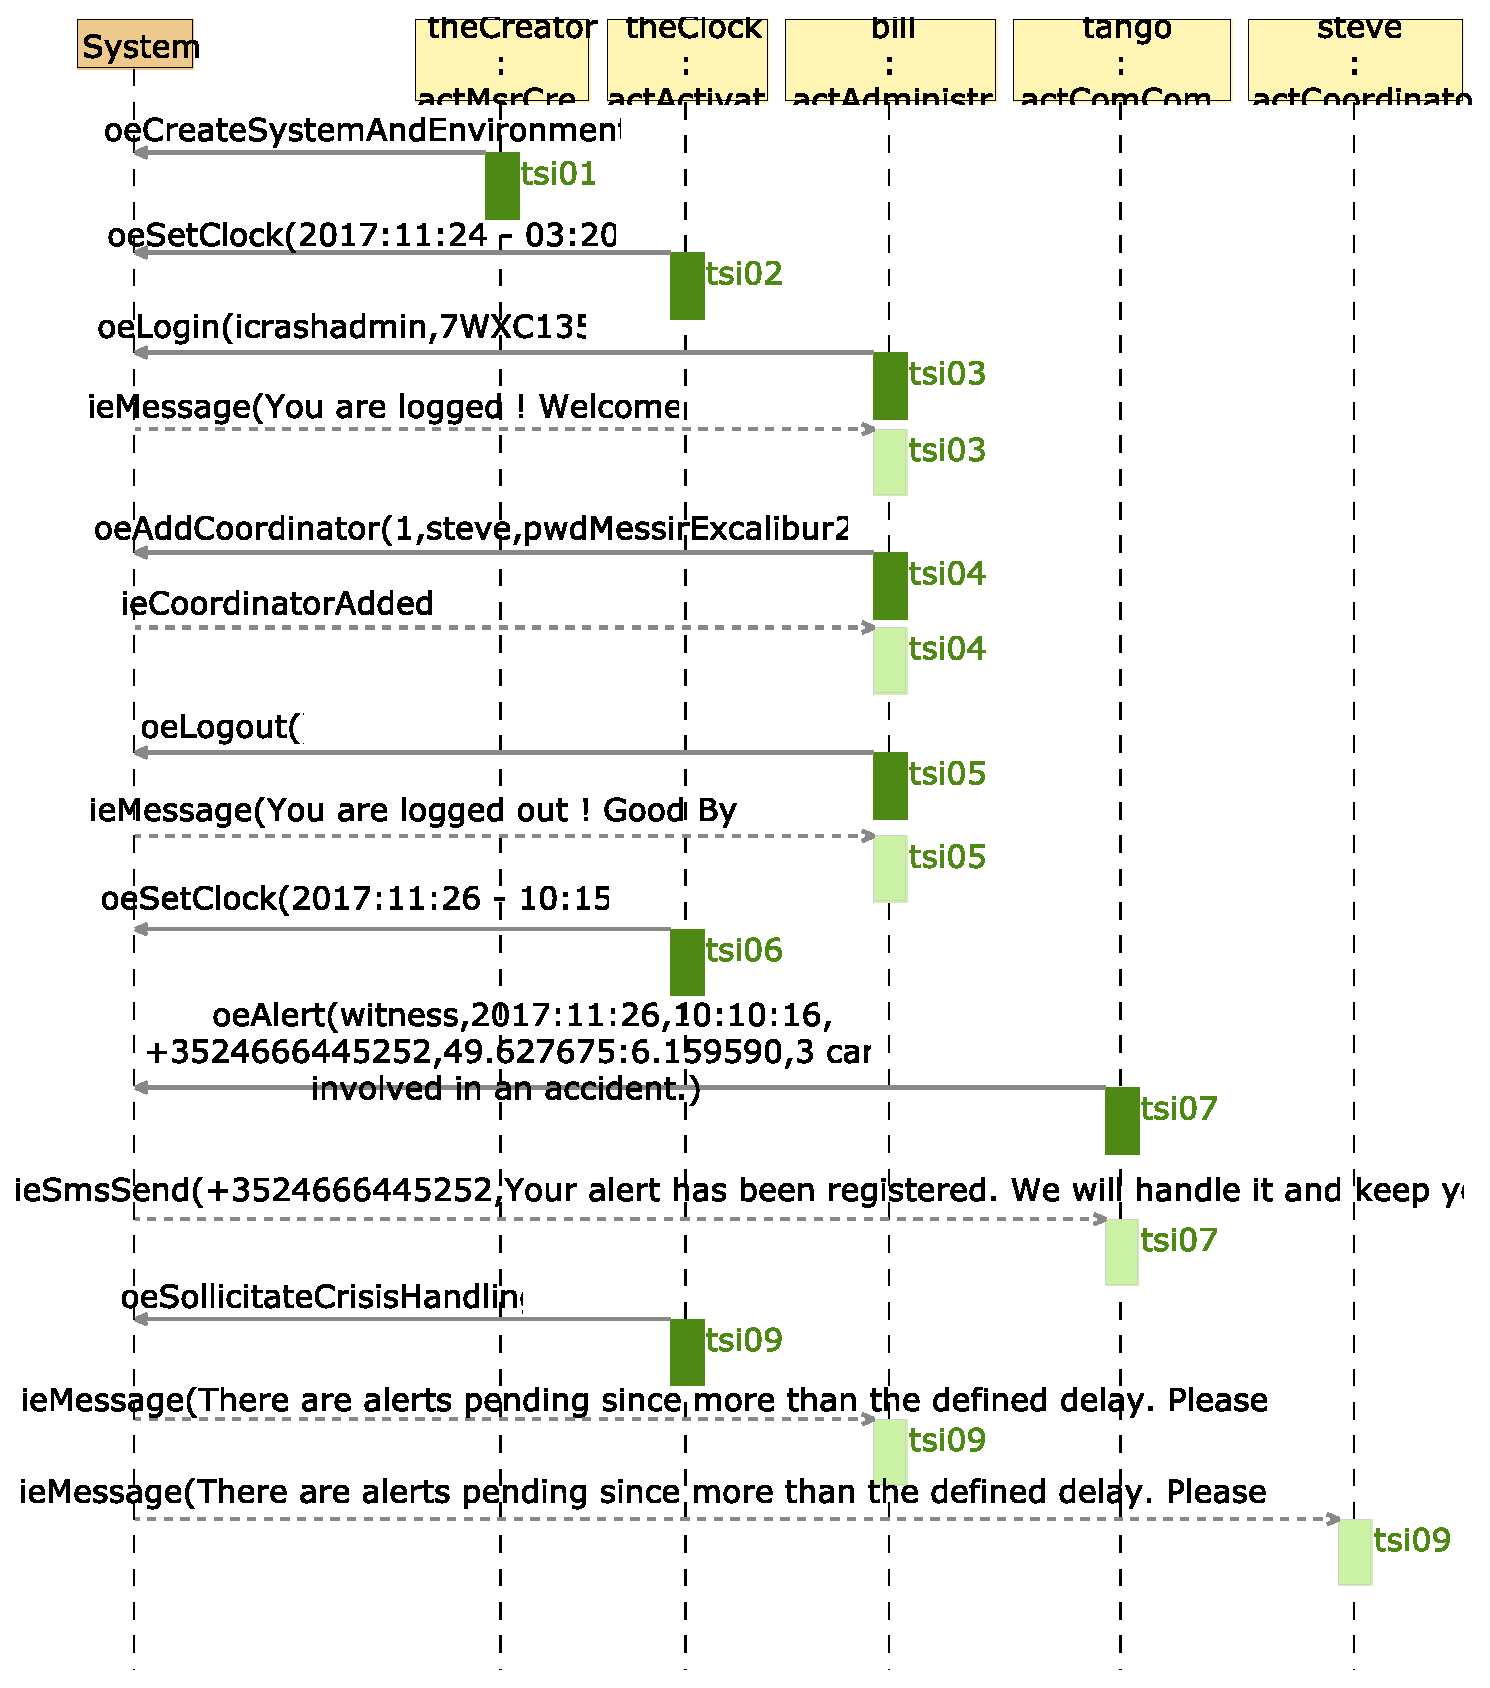
\includegraphics[angle=0
,width=1.0\textwidth
]{./images-report-gen/testcase-model/tci-testcase01-instance01-Part01.eps}
\end{center}
\caption[lu.uni.lassy.excalibur.examples.icrash Sequence Diagram: tci-testcase01-instance01-Part01]{tci-testcase01-instance01-Part01 testcase instance sequence diagram
}
\label{fig:lu.uni.lassy.excalibur.examples.icrash-TM-instanceview-tci-testcase01-instance01-Part01}
\end{figure}
\vspace{0.5cm}

\subsection{Test Case Instance - instance01Part02}


%%%%%%%%%%%%%%%%%%%%%%%%%%%%%%%%%%%%%%%%%%%%%%%%%%
%Test Step Instances
%%%%%%%%%%%%%%%%%%%%%%%%%%%%%%%%%%%%%%%%%%%%%%%%%%


Figure \ref{fig:lu.uni.lassy.excalibur.examples.icrash-TM-instanceview-tci-testcase01-instance01-Part02}
Sequence diagram representing the second part of a simple and complete testcase instance for \msricrash.

\begin{figure}[htbp]
\begin{center}

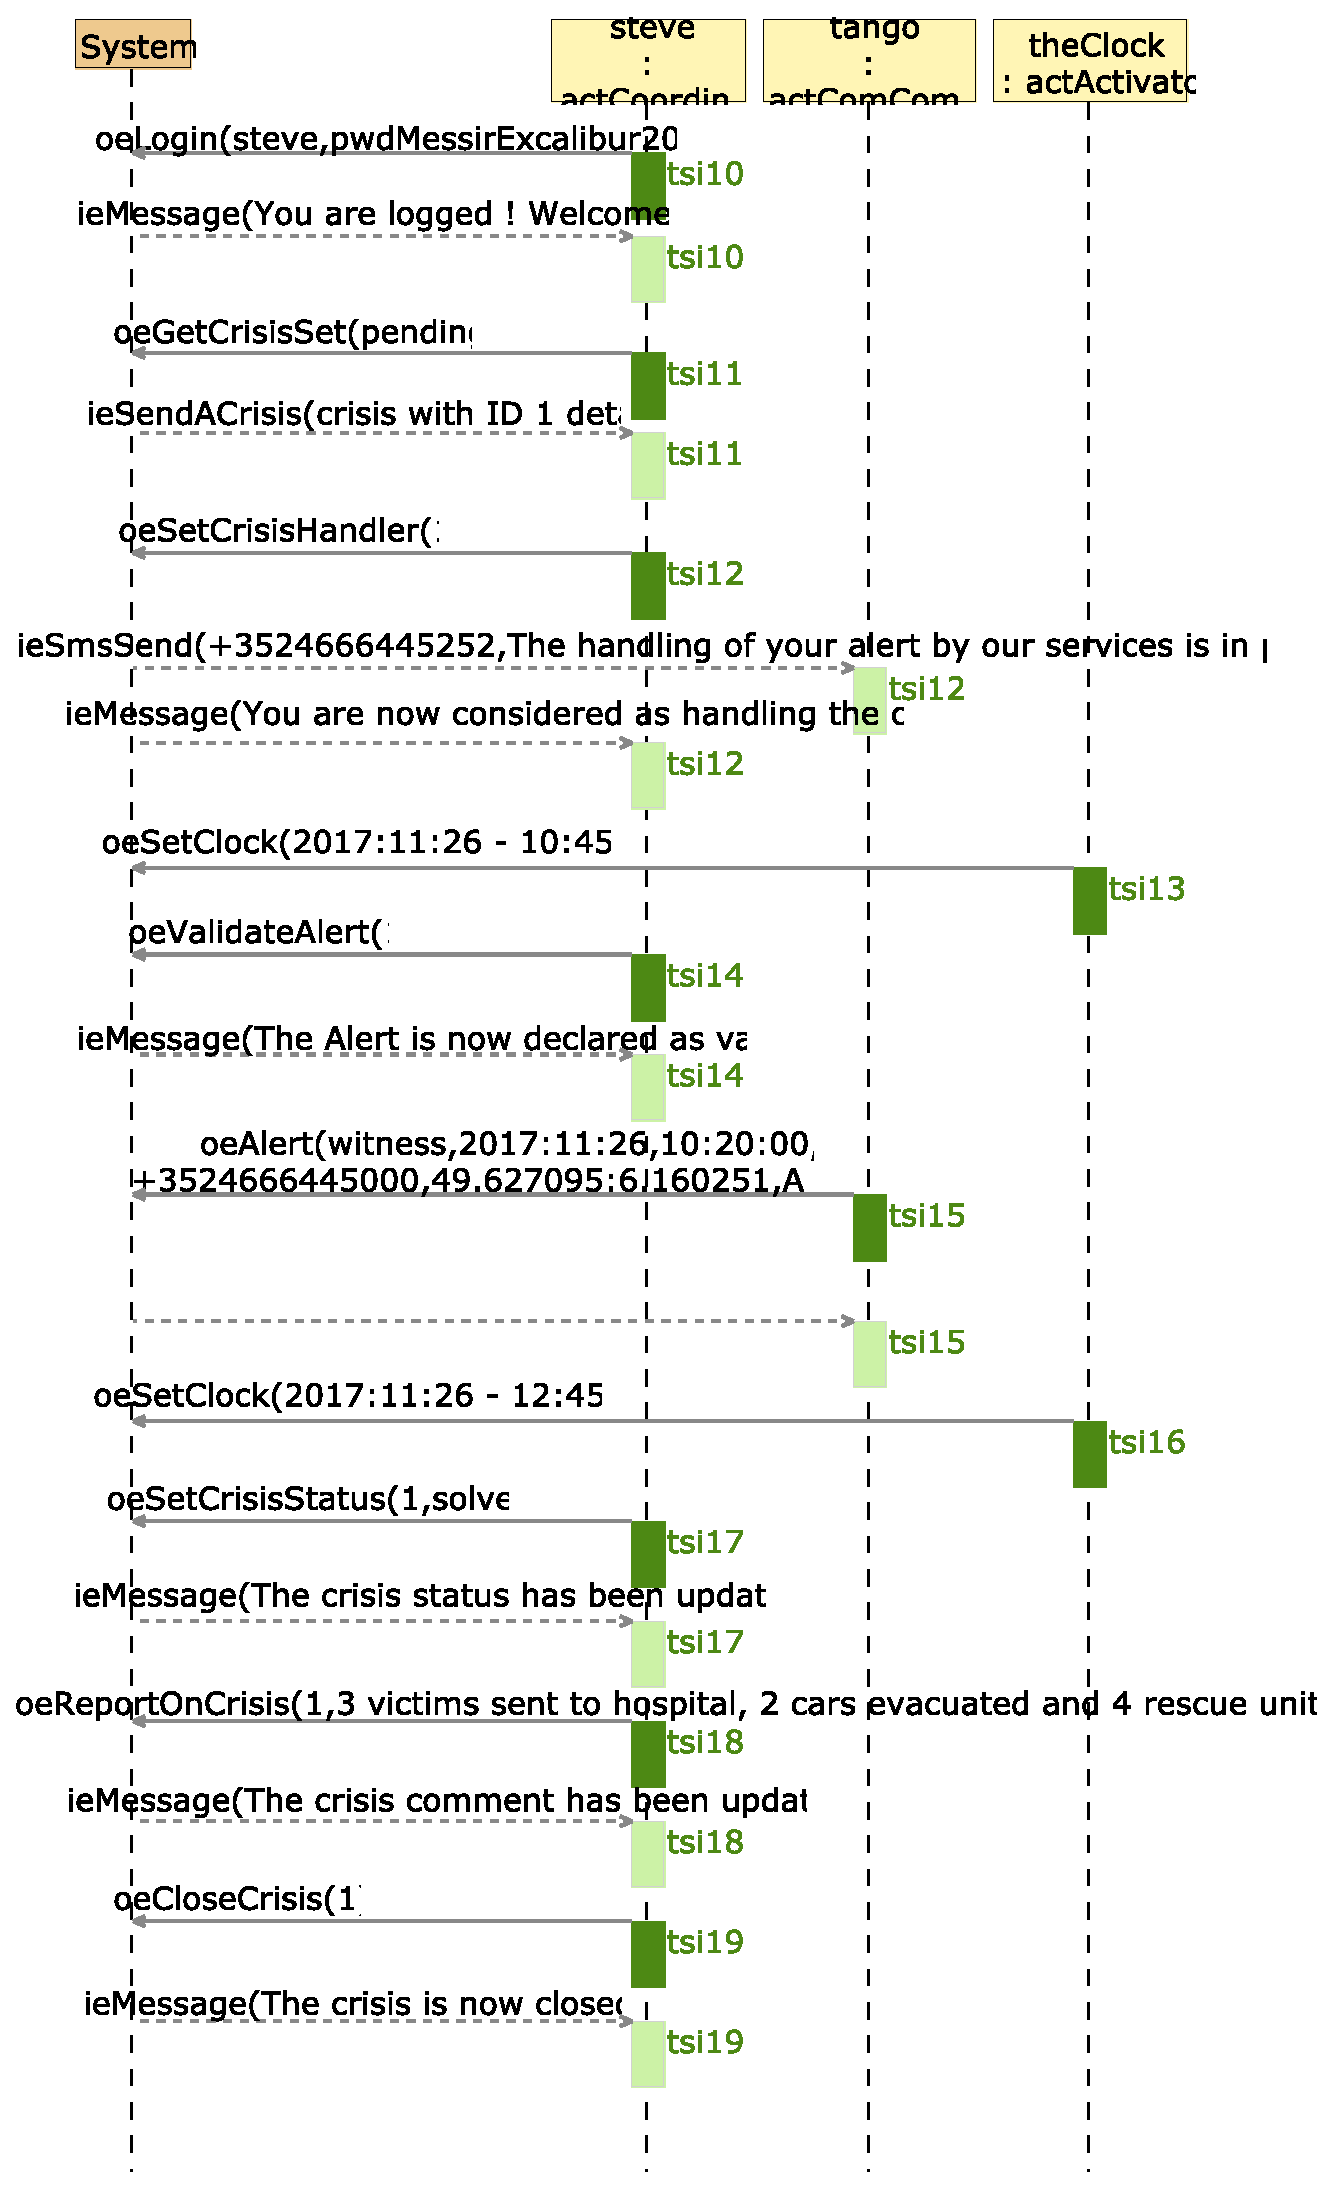
\includegraphics[angle=0
,height=1.0\textheight
]{./images-report-gen/testcase-model/tci-testcase01-instance01-Part02.eps}
\end{center}
\caption[lu.uni.lassy.excalibur.examples.icrash Sequence Diagram: tci-testcase01-instance01-Part02]{tci-testcase01-instance01-Part02 testcase instance sequence diagram
}
\label{fig:lu.uni.lassy.excalibur.examples.icrash-TM-instanceview-tci-testcase01-instance01-Part02}
\end{figure}
\vspace{0.5cm}





